\section{Selection}

This analysis uses all the \pp collision data in Run 1 and Run 2 stage, 
corresponding to an integrated luminosity of $3\invfb$ ($6\invfb)$ in Run 1 (Run 2). 
The simulation samples of the $\Lb\to\jpsi\proton\Km$ decay are generated by \pythia with $pp$ collisions at $\sqrt{s}=7\tev$, $8\tev$ and $13\tev$ respectively,
with the ratio of the numbers of events roughly one to two between Run 1 and Run 2.
Both \pythia6 and \pythia8 generators are used.
The Monte Carlo event type is \texttt{15144001}, 
in which $\Lb$ is forced to decay into the $\jpsi\proton\Km$ final state with the PHSP model.

%
\subsection{Reconstruction and pre-selection}
In this analysis the reconstruction of the \Lb candidate starts
from the stripping line \texttt{FullDSTDiMuonJpsi2MuMuDetachedLine} in the \texttt{DiMuon} stream 
of the stripping reconstruction,
which different version, 
\texttt{S21r1} for 2011, 
\texttt{S21} for 2012, 
\texttt{S24} for 2015, 
\texttt{S28} for 2016, 
\texttt{S29r2} for 2017, 
and \texttt{S34} for 2018. 
The selection criteria in this stripping line is summarized in Table~\ref{tab:JpsiSelection_jpsipk}.
The \jpsi candidate is formed by two oppositely charged tracks consistent with muon hypotheses (IsMuon) 
with $\pt>550\mevc$ and good track fit quality $\chisqndf<4$.
The $\jpsi$ candidate is required to have an invariant mass within the $\pm100\mevcc$ window 
around the know \jpsi mass~\supercite{PDG2014}, and to have a vertex fit quality $\chisqvtx<20$.
The $\jpsi$ candidate is consistent with originating from $b$-hadron decays by requiring its decay length significance (DLS) to be greater than three.

%
Conparing to the previous study\supercite{LHCb-PAPER-2015-024},
the selection criteria is optimized,
all differences between the new selection criteria and old study are summarized in Table~\ref{tab:PreSelection_jpsipk}.
To select good $\jpsi$ candidates,
a tightened PID cut $\dllmupi>0$ is required for both muon tracks in the final state,
and the dimuon invariant mass window is reduced to $[-48,\,43]\mevcc$ around the known \jpsi mass~\supercite{PDG2020}.
The \jpsi mass resolution is around $13\mevcc$.
To reconstruction the \Lb candidate, 
the $\jpsi$ candidate is combined with two opposite charged tracks, 
consistent with pions and protons respectively.
This is achieved by PID cuts on the \ProbNN variables: $\ProbNN_{K}(K)>0.2$ and $\ProbNN_{p}(p)>0.2$.
The two hadronic tracks are required to have large transverse momenta, $\pt>250\mevc$,
inconsistent with originating from the primary vertex (PV), $\chisqip>9$.
%The $\Lb$ candidate is required to have a displayed decay vertex, $\chisq_\tau>9$, with good vertex fit quality, $\chisqndf<10$.
The $\Lb$ candidate is required to have a good vertex fit quality, $\chisqndf<10$,
with a displayed decay vertex,
flight distance to primary vertex is larger than $1.5$\mm.
It should be consistent with being produced from PV by requiring $\chisqip<25$ and cosine value of the direction angle, DIRA$>0.999$.
And the \chisq of closet approach distance between \proton and \Km is smaller than 16.
The $\Lb$ candidates with mass $5.1<M(\jpsi p\pi^-)<6.5 \gevcc$ are selected.

The $\Lb\to\jpsi\proton\Km$ decay chain is refitted with two sequential constraints using the \texttt{DecayTreeFitter} to improve the mass resolution:
A) the \jpsi candidate mass constrained to its known value~\supercite{PDG2020} and
the $\Lb$ candidate constrained to originating from the PV;
B) the invariant mass of the $\Lb$ candidate constrained to its know value~\supercite{PDG},
with the momenta of the $\jpsi$, $p$ and $\Km$ daughters re-calculated according to this constraint.

It should be noted that the PID requirements on the hadron tracks are not applied when reconstructing the $\Lb$ candidates in the simulation sample.
The effect, instead, is considered using weights from the PID calibration (\texttt{PIDCalib}).
The pion track is calibrated using pion tracks from the $\Dstar$ tagged $\decay{\Dz}{\Km\pip}$ decay,
while the proton track is calibrated using proton tracks from the $\decay{\Lc}{p\Km\pip}$ decay.

Events with $\Lb$ candidates in both the simulation and the data samples are required to fire (TOS) the trigger sequences:
%at the \lone level by either of the \texttt{L0Muon} and \texttt{L0DiMuon} lines; 
at the \hltone level by either of the \texttt{Hlt1DiMuonHighMass}, \texttt{Hlt1TrackMuon} and \texttt{Hlt1TrackAllL0} for Run 1 sample,
while \texttt{Hlt1DiMuonHighMass}, \texttt{Hlt1TrackMuon}, \texttt{Hlt1TwoTrackMVA} and \texttt{Hlt1TrackMVA} for Run 2 sample;
and at the \hlttwo level by either of
the \texttt{Hlt2DiMuonDetachedJPsi} lines.


%%%%%%%%%%%%%%%%%%%%%%%%%%%%%%%%%%%%%%%%%%%%%%%%%%%%%%%%%%%%%%%%%%%%%%%%%%%%%%%%%%%%%%%%%%%%%%%%%%%%%%%%%%%%%%%%%%%%%%%
\begin{table}[tbh]
\caption{Stripping selections of $\jpsi$ candidates in the line \texttt{FullDSTDiMuonJpsi2MuMuDetachedLine}.}
\centering
\begin{tabular}{rl}
\hline
Quantity               & Selections \\
\hline
IsMuon$(\mu)$          & $=$ TRUE \\
DLL$(\mu-\pi)$     & $>$ 0\\
$\pt(\mu)$             & $>550\mevc$ \\
Track $\chisqndf(\mu)$ & $<4$  \\
$\Delta M(\jpsi)$      & $<100\mevcc$\\
Vertex $\chisq(\jpsi)$ & $<20$ \\
DLS($\jpsi$)           & $>3$  \\
\hline
\end{tabular}
\label{tab:JpsiSelection_jpsipk}
\end{table}
%%%%%%%%%%%%%%%%%%%%%%%%%%%%%%%%%%%%%%%%%%%%%%%%%%%%%%%%%%%%%%%%%%%%%%%%%%%%%%%%%%%%%%%%%%%%%%%%%%%%%%%%%%%%%%%%%%%%%%%

\begin{table}[tbh]
\caption{Pre-selections of $\LbJpsiPPi$ candidates between old Run 1 analysis and this one.}
\centering
\begin{tabular}{c c | c c}
\hline
    & Quantity               & Old Run 1 & This analysis \\
\hline
1   & All tracks \chisqndf   & $<4$             		& same  \\
2   & clone track rejection  & CloneDist cut    		& same \\ 
3   & ghose rejection        & ghost probability < 0.2	& same \\ 
2   & muon DLL(\muon)        & $>0$\&ISMUON     		& same  \\
5   & vertex of \jpsi        & $\chisq<16$      		& same  \\
6   & mass window of\jpsi    & $[-48,43]\mev$   		& same  \\
3   & \pt of muon            & $>550\mev$       		& $>500\mev$  \\
4   & \pt of hadron          & $>250\mev$       		& same  \\
4   & \pt(\proton)+\pt(\Km)& $>900\mev$                     & same  \\
7   & \chisqvs of hadron     & $>9$             		& same  \\
8   & PID of $\kaon$         & DLL($\kaon-\pi$)>0 and DLL($\proton-\kaon$)<3       & ProbNNk$>0.2$  \\
9   & PID of \proton         & DLL($\proton-\pi$)>10 and DLL($\proton-\kaon$)>3    & ProbNNp$>0.2$  \\
16   & DOCA \chisq of \proton\Km   & $<16$               	& same \\
11   & \Lb vertex             & $\chisqvtxndf<10$     	& same  \\
10   & \chisqip of \Lb        & $<25$                 	& same  \\
12   & DIRA of \Lb            & $>0.999$             		& same \\
15   & Flight distance of \Lb       & $>1.5\mm$             & same \\
\hline
\end{tabular}
\label{tab:PreSelection_jpsipk}
\end{table}
%%%%%%%%%%%%%%%%%%%%%%%%%%%%%%%%%%%%%%%%%%%%%%%%%%%%%%%%%%%%%%%%%%%%%%%%%%%%%%%%%%%%%%%%%%%%%%%%%%%%%%%%%%%%%%%%%%%%%%%



%\subsection{Reflections vetoing}
%%Since the decays of $\Bd\to\jpsi K\pi$, $\Bs\to\jpsi K K$, $\B^0_{(\squark)}\to\jpsi\pi\pi$, 
%Since the decays of $\Bd\to\jpsi K\pi$, $\Bs\to\jpsi\Kp\Km$,
%$\LbJpsipK$ have much larger branching fractions than the \LbJpsippi decay,
%even after the PID requirements on the hadron tracks,
%the \LbJpsippi sample is still potentially contaminated by these decays.
%To investigate the effects of the reflections from these decays,
%the invariant mass of the \Lb candidate in the \LbJpsippi sample is re-calculated
%with the proton assumed as a pion or kaon and/or the pion assumed as a kaon or proton.
%Figure~\ref{fig:Reflections} shows
%these re-calculated invariant mass distributions for those \LbJpsippi candidates
%within the $\pm20\mevcc$ mass window ($\approx3\sigma)$) around the known \Lb mass\supercite{PDG2020}.
%Clear contamination with the $\Bd\to\jpsi K\pi$, $\Bs\to\jpsi K K$ and $\LbJpsipK$ decays are observed,
%as shown by the narrow peaks around the known $\Bd$, $\Bs$ and $\Lb$ masses in the top right,
%bottom left and bottom middle plots in Fig.~\ref{fig:Reflections}.
%The contribution of $B^0_{(\squark)}\to\jpsi\pi\pi$ decays is insignificant.
%The contamination from $\Bd\to\jpsi K\pi$ is vetoed if:
%$M(\jpsi [\proton\to K]\pi)$ sits in the $\pm22\mevcc$ window around the known $\Bz$ mass\supercite{PDG2020},
%or $M(\jpsi [\proton\to\pi][\pi\to K])$ sits in the $\pm22\mevcc$ window around the known $\Bz$ mass
%and ProbNNpi(\proton)$>0.1$\&ProbNNk($\pi$)$>0.1$.
%The contamination with the \LbJpsipK decay is vetoed if:
%$M(\jpsi \proton[\pim\to K])$ sits in the $\pm22\mevcc$ window around the known $\Lb$ mass\supercite{PDG2020}
%and ProbNNk($\pi$)$>0.2$,
%or $M(\jpsi [\proton\to K][\pi\to\proton])$ sits in the $\pm22\mevcc$ window around the known $\Bz$ mass
%and ProbNNk(\proton)$>0.1$\&ProbNNp($\pi$)$>0.1$.
%Besides,
%the reflection of $\Bs\to\jpsi\Kp\Km$ decay is removed in this case:
%$M(\jpsi [\proton\to K][\pim\to K])$ sits in the $\pm22\mevcc$ window around the known $\Bs$ mass\supercite{PDG2020}.
%
%
%A large fraction of \LbJpsippi candidates come from the decay $\decay{\Lb}{\jpsi\Lambda^0}$ with $\decay{\Lambda^0}{p\pi^-}$,
%which is not interesting in this analysis.
%These events are removed if the invariant mass $M(p\pim)$ locates in the $\pm 5\mevcc$ window around the known $\Lambda^0$ mass~\supercite{PDG2020}.
%
%During the invariant mass vetoing,
%the mass resolutions are determined by fitting the invariant mass distribution in a narrow region around the signal peak;
%the signal mass shape is described by double-sided crystal ball function (DSCB) with tail parameters fixed to
%the $\LbJpsiPPi$ simulation,
%while the background is simply described by a linear function.
%
%%%%%%%%%%%%%%%%%%%%%%%%%%%%%%%%%%%%%%%%%%%%%%%%%%%%%%%%%%%%%%%%%%%%%%%%%%%%%%%%%%%%%%%%%%%%%%%%%%%%%%%%%%%%%%%%%%%%%%%%
%\begin{figure}[!tbh]
%\centering
%\begin{minipage}[t]{1.0\textwidth}
%\centering
%\includegraphics[width=0.3\textwidth]{Figures/04_Penta/02_selection/draw_veto_pic/Lb_mass_P2K}
%\includegraphics[width=0.3\textwidth]{Figures/04_Penta/02_selection/draw_veto_pic/Lb_mass_P2Pi}
%\includegraphics[width=0.3\textwidth]{Figures/04_Penta/02_selection/draw_veto_pic/Lb_mass_PPi2KK} \\
%\includegraphics[width=0.3\textwidth]{Figures/04_Penta/02_selection/draw_veto_pic/Lb_mass_PPi2KP}
%\includegraphics[width=0.3\textwidth]{Figures/04_Penta/02_selection/draw_veto_pic/Lb_mass_PPi2PiK}
%%\includegraphics[width=0.3\textwidth]{Figures/04_Penta/02_selection/draw_veto_pic/Lb_mass_PPi2PiP} \\
%\includegraphics[width=0.3\textwidth]{Figures/04_Penta/02_selection/draw_veto_pic/Lb_mass_Pi2K}
%   %\put(-120,230) {\textrm{\small\bf {LHCb Unofficial} }}\\
%   %\put(-120,230) {\textrm{\small \bf \color{red}{ LHCb Unofficial} }}\\
%\end{minipage}
%\caption{
%  Invariant mass distributions of the \LbJpsippi candidate with the $p$ and the $\pim$ assumed to be other hadrons
%   for those \Lb candidates in the $\pm20\mevcc$ mass window around the know \Lb mass.
%  The lablels $\hadron\to\hadron'$ indicate that the \hadron hadron in the \LbJpsippi decay is assumed as a $\hadron'$ hadron.
%}
%\label{fig:Reflections}
%\end{figure}
%%%%%%%%%%%%%%%%%%%%%%%%%%%%%%%%%%%%%%%%%%%%%%%%%%%%%%%%%%%%%%%%%%%%%%%%%%%%%%%%%%%%%%%%%%%%%%%%%%%%%%%%%%%%%%%%%%%%%%%%




\subsection{Multivariate analysis}

The multivariate analysis (MVA) is used to further suppress the background.
%In the MVA training the signal sample is from the $\LbJpsiPPi$ simulation using the PHSP model,
%while the background sample is from the upper sideband of the $\LbJpsiPPi$ invariant mass distribution,
%$M(\jpsi p\pi)\in[5.67,5.80]\gevcc$.
%These samples are randomly split into two halves, one for the training and the other for the test.
%Different from the previous study,
%the PID information variables are included in the MVA classification.
%All used variables are listed it Table.~\ref{tab:MVA}
%The smaller value of the two muon PID variables ($\dllmupi$);
%the smaller value of the $\chisqip$ of the two muon tracks;
%the smaller value of the $\chisqip$ of the two hadron tracks;
%the arithmetic addition of the \pt of the two hadrons;
%the DIRA, the flight distance (FD), the $\pt$, the $\chisqip$ and the vertex fit quality ($\chisqvtxndf$) of the $\Lb$ candidate.
%the PID varibles of hadrons.
All variables used are listed in Table.~\ref{tab:MVA_jpsipK}.
Besides,
the Run 1 and Run 2 samples are studied seperately.
The distributions of these variables of Run 2 sample for the signal in the simulation sample and the background in the data sideband
are shown in Figure.~\ref{fig:MVAvairables},

\begin{table}[tbh]
\caption{Variables used in TMA study.}
\centering
\begin{tabular}{c | c }
\hline
    & Variables    \\
\hline
1   & \chisqvtx of \Lb \\
2   & $log(1-cos\theta_{p})$      \\
3   & \chisqip of \Lb     \\
4   & min \chisqip of hadron \\
5   & FD of \Lb		\\
6   & \pt of \Lb 		\\
7   & sum \pt of hadrons \\
8   & min PID of muon	\\
9   & ProbNNp of \proton \\
10  & ProbNNk of \Km  \\
11  & momentum of \proton   \\

\hline
\end{tabular}
\label{tab:MVA_jpsipK}
\end{table}


\begin{figure}[!tbh]
\centering
\begin{minipage}[t]{1.0\textwidth}
\centering
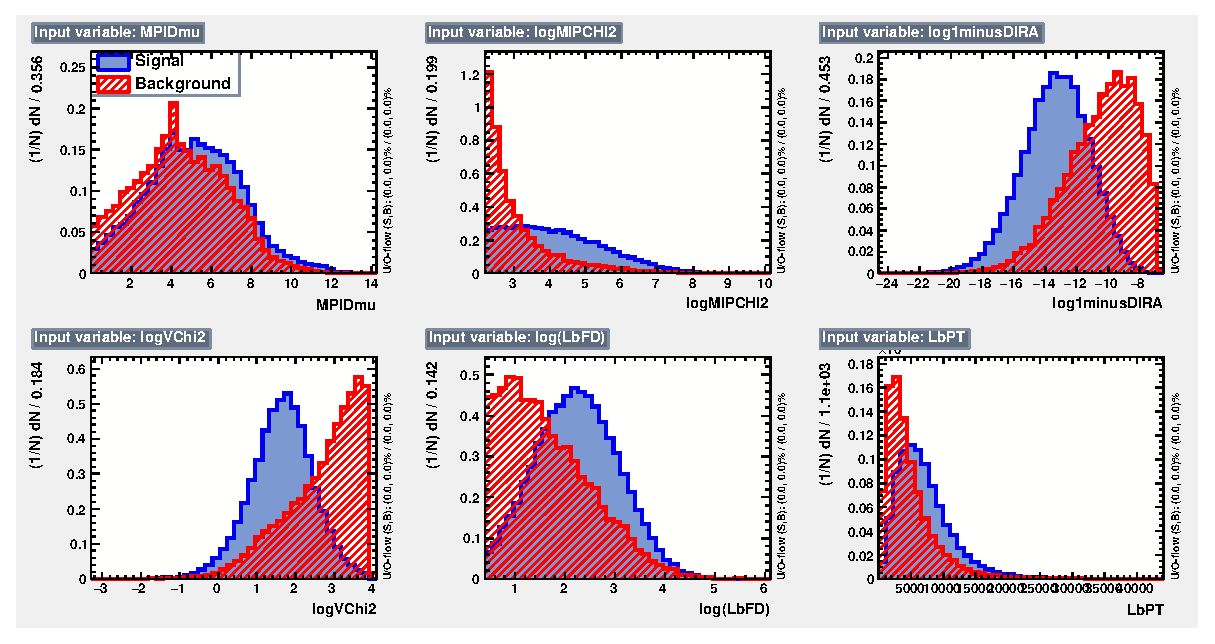
\includegraphics[width=0.95\textwidth]{Figures/08_JpsipK/mva_plots/variables_id_c1.eps} \\
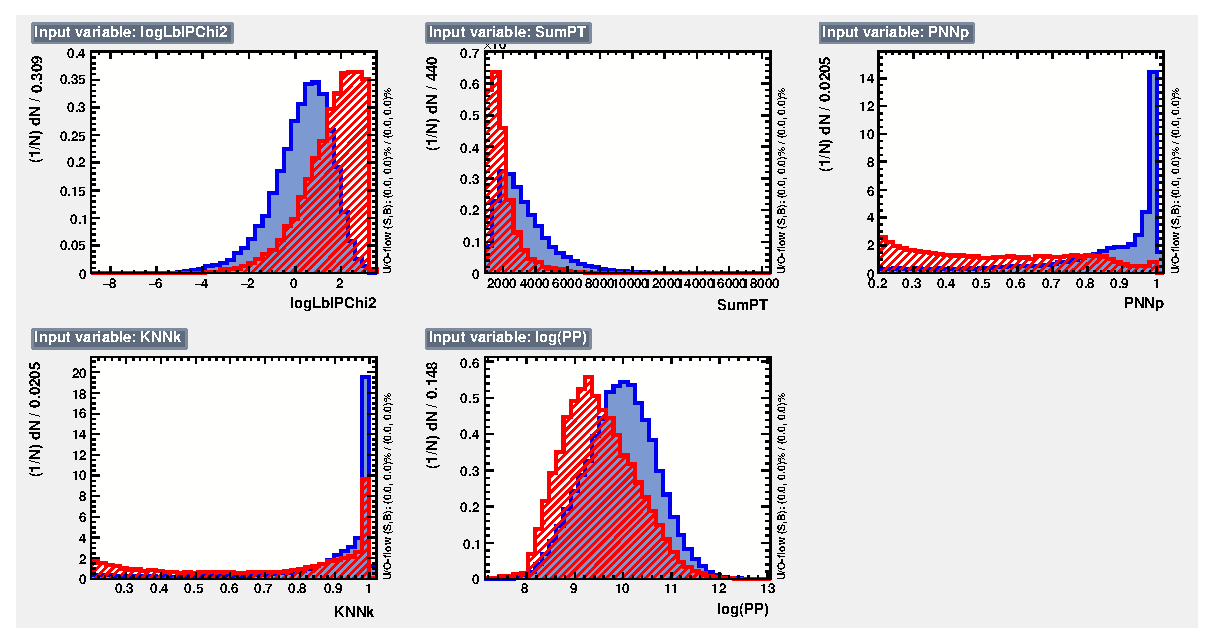
\includegraphics[width=0.95\textwidth]{Figures/08_JpsipK/mva_plots/variables_id_c2.eps}
\end{minipage}
\caption{Discriminating variables used in the MVA training of Run 2 sample.}
\label{fig:MVAvairables}
\end{figure}

%The ROC curves of the results of different training methods are given in the left plot of Fig.~\ref{fig:MVAMonitor}.
The BDTG method is used as the default method,
and the overtraining test for the BDTG method is given in the right plot of Figure.~\ref{fig:MVAMonitor} for Run 2 samples.
The BDTG discriminant distributions for the training samples are consistent with those in the test samples.
No effect of overtraining is observed.
The working point of the BDTG value is optimized by maximizing the figure of merit (FoM) of the signal significance,
defined as $S/\sqrt{S+B}\times\epsilon_{S}$.
The $\epsilon_S$ is the signal efficiency for a specified BDTG cut and is determined from the simulation sample,
while $S$ ($B$) is the number of the signal (background) events in the $\pm3\sigma$ region around the known $\Lb$ mass
in the $\jpsi\proton\pi$ invariant mass distribution of the data.
%It should be noted that the PID requirements on the $p$ and $\pi$ need also to be tightened on top of the pre-selection.
%However, 
%it is found that the BDTG cut value that maximizes the FoM doesn't depends strongly on the PID cuts of the two hadron tracks.
%In Figure.~\ref{fig:BDTGCut},
The distribution of the FoM as a function of the BDTG cut value is given,
and the value of $0$ for Run 1 and $-0.4$ for Run 2 are determined as the default working points.


%%%%%%%%%%%%%%%%%%%%%%%%%%%%%%%%%%%%%%%%%%%%%%%%%%%%%%%%%%%%%%%%%%%%%%%%%%%%%%%%%%%%%%%%%%%%%%%%%%%%%%%%%%%%%%%%%%%%%%%
\begin{figure}[!tbh]
\centering
\includegraphics[width=0.48\textwidth]{Figures/08_JpsipK/mva_plots/overtrain_BDTG.eps}
%\includegraphics[width=0.48\textwidth]{Figures/04_Penta/02_selection/tmva/plots_run2/overtrain_BDTG}
\caption{
   The BDTG output distribution for signals and the background in the training sample and the test sample of Run 2 sample.}
\label{fig:MVAMonitor}
\end{figure}

%\begin{figure}[!tbh]
%\centering
%\includegraphics[width=0.48\textwidth]{Figures/04_Penta/02_selection/tmva/plots_run1/mvaeffs_BDTG}
%\includegraphics[width=0.48\textwidth]{Figures/04_Penta/02_selection/tmva/plots_run2/mvaeffs_BDTG}
%   \caption{Signal significance (arbitrary unit) for different BDTG cut values of Run 1(left) and Run 2(right) samples.}
%\label{fig:BDTGCut}
%\end{figure}
%%%%%%%%%%%%%%%%%%%%%%%%%%%%%%%%%%%%%%%%%%%%%%%%%%%%%%%%%%%%%%%%%%%%%%%%%%%%%%%%%%%%%%%%%%%%%%%%%%%%%%%%%%%%%%%%%%%%%%%%














